%!TEX program = xelatex
% 完整编译方法 1 pdflatex -> bibtex -> pdflatex -> pdflatex
% 完整编译方法 2: xelatex -> bibtex -> xelatex -> xelatex
\documentclass[lang=cn,11pt,authoryear]{elegantpaper}

\title{银行存管、投资者决策与 P2P 网络借贷规范发展\footnote{本文为~\href{https://github.com/ElegantLaTeX/ElegantPaper}{ElegantPaper} 的示例文档,最新版\href{https://github.com/EthanDeng/bank-custody}{下载}。}}
\author{\href{http://www.cces.fudan.edu.cn/researchdetail.aspx?id=6}{陈钊} \quad \href{https://ddswhu.me/}{邓东升}}

\institute{复旦大学 \; 经济学院\\ 中国社会主义市场经济研究中心}
\date{2019 年 6 月 13 日}


\begin{document}

\maketitle

\begin{abstract}
为了避免网贷平台触碰资金,降低网贷行业道德风险,监管部门要求网贷平台必须与银行签订存管协议,平台只能作为信息中介撮合投资者和借款人。利用网贷平台银行资金存管信息和网贷平台的微观运营数据,通过对于银行存管对于网贷平台和网贷投资者的影响的实证研究发现,作为衡量平台资金安全的重要措施 —— 银行存管确实能为网贷平台提供增信作用,投资者更愿意投资进行了资金存管的平台。平台通过与银行签订存管协议能够向投资者提供一个信号,让网贷平台更加可信。但是,实证研究表明,只有当平台的全部借贷业务都上线了资金存管,平台的运营才真正接近于纯粹的信息中介。
\keywords{P2P 网络借贷 \; 银行存管 \; 信息中介}
\end{abstract}

\section{我国 P2P 网络借贷的发展}
我国 P2P 网贷的发展根据行业特征可以划分为三个发展阶段,分别是:萌芽期(2007 -- 2013),野蛮生长期(2013 -- 2016 年 8 月),合规监管期(2016 年 8 月至今)\footnote{对网贷行业的发展阶段的划分,参考了网贷之家上的分析文章《\href{https://www.wdzj.com/zhuanlan/guancha/17-10089-1.html}{盘点 P2P 行业 11 年发展史——从野蛮到合规的辛酸历程》},并根据制度环境的变化进行了一定的调整。}。

2007 年,国内首家 P2P 网络借贷平台 —— 人人贷在上海成立,揭开了我国 P2P 网络借贷行业发展的序幕。早期,以信用借款为主的网络借贷发展比较缓慢,网贷平台数和网贷借款人、投资者都非常少,2007 至 2013 年被称为网贷的萌芽期。

直到 2013 年左右,商业银行收缩贷款~\citep{pmm2014},网贷行业获得了巨大生机,P2P 网贷进入了“野蛮生长”阶段。在此期间,网络借贷平台数量,网络借贷的借款人和投资者数量都获得了爆炸性增长。根据网贷行业最大的门户网站 —— \href{https://www.wdzj.com/}{网贷之家}\footnote{网贷之家是中国 P2P 业内最大、最权威、最具影响力的行业门户,汇集了较多 P2P 平台的运营数据。据我们所知,此网站数据是国内 P2P 平台运营数据唯一可得的来源,且覆盖面最广。}的数据,截止到 2015 年 9 月,网贷行业的月度成交量超过了 1000 亿元,同期月度投资者达到了 240 万人,月度借款人约 57 万人\footnote{资料来源:网贷之家研究院,《\href{https://www.wdzj.com/news/baogao/16305.html}{网贷之家发布 2014 年中国网贷行业年报(完整版)}》,2015 年 1 月 6 日。}。

而伴随着网贷行业的扩张,征信不足,监管缺失的问题逐渐显现出来。2015 年,网络借贷平台频繁爆发跑路问题,2015 年一整年新增近 1300 家问题平台\footnote{问题平台定义:平台出现无法提现、跑路、停业、经侦介入等,均被定义为问题平台,否则视为正常平台。},是 2014 年及以前总和的近 3 倍。同年 12 月 16 日,互联网金融平台 e 租宝涉嫌犯罪,被立案侦查。根据网贷之家的数据,截至 12 月 8日,e 租宝总成交量 745.68 亿元,总投资人数 90.95 万人,待收总额 703.97 亿元。2016 年 1 月警方公布 e 租宝非法集资 500 多亿。

2015 年 1300 家问题平台的爆发也让网络借贷行业在社会上受到了前所未有的关注,网贷行业迫切需要政府制定监管政策,2015 年 12 月,政府发布《网络借贷信息中介机构业务活动管理暂行办法(征求意见稿)》,并于 2016 年 8 月正式发布该办法。以 8 月 24 日《网络借贷信息中介机构业务活动管理暂行办法》\footnote{《网络借贷信息中介机构业务活动管理暂行办法》被称为网贷“基本法”。}正式发布为节点,网贷行业进入合规监管阶段。

《暂行办法》虽然对于网贷机构的设立不设行政许可,采取无条件备案的方式,但通过设置单一借款人上限要求以及负面清单管理等措施来规范和约束网贷机构,防范相关风险。《暂行办法》也明确规定平台只能作为信息中介撮合投资者与借款人,并对资金的安全性进行了界定,规定平台为了合规备案需要进行资金存管,避免平台发生自融。而在此之后,为了更好的引导平台的进行合规备案,针对《暂行办法》提到的备案制度、资金存管以及信息披露相应出台了三项具体的指引细则\footnote{ 分别是《网络借贷信息中介机构备案管理登记指引》(“备案指引”),《网络借贷资金存管业务指引》(“存管指引”)与《网络借贷信息中介机构业务活动信息披露指引》(“信披指引”),与《暂行办法》合称“1 + 3”网贷监管体系。}。

“1 办法 + 3 指引”构成的网贷监管体系形成之后,也标志着 P2P 网贷正式进入合规监管的进程。在《暂行办法》发布之后,平台被要求从金融(信用)中介向完全信息中介转型,并且网贷行业从监管缺失变成备案准入制。由于银行存管是网贷备案的基础条件之一且该要求对平台影响重大,下文将实证检验《暂行办法》对网贷机构银行存管的要求对于网贷行业和投资者的影响。目前国内较多的研究只是涉及到对网贷行业风险及可能的监管对策的讨论~\citep{lsq2014,wj2015,awhxmy2016},但是,围绕网贷行业的监管政策开展的实证研究非常少见。

例如,\cite{gf2016a} 与~\cite{tym2017} 分别透过金融央地关系视角总结了中国 P2P 网络借贷平台的地区特征,特别是风险特征和现有监管手段的有效性,并提出了一些针对性的政策建议。\cite{xsypylwyq2018} 采用人人贷平台的微观数据样本,从实证角度研究行业监管中关于平台中介性质要求的有效性。\cite{lsxlh2015} 使用了网贷之家 59 个平台的 5 个月面板数据,研究了风险投资、第三方资金托管对 P2P 网络借贷平台成交量的影响。但是,这项研究的数据量比较小,并且由于数据时间跨度比较短,在他们样本中,平台是否有第三方作为资金托管方基本上在样本内处于恒定不变,这就难以在控制平台固定效应的同时考察资金托管对平台的影响。

导致这方面实证研究较为缺乏的原因之一是很多平台的数据并不公开,即便是网贷行业最大的门户网站 —— 如网贷之家或\href{https://www.p2peye.com/}{网贷天眼},所提供的运营数据也非常有限。这就限制了当前对于网贷平台运营风险以及监管政策评价的微观计量研究。

所幸的是,在部分数据下线之前作者就已经通过 Python 爬虫获得了网贷之家 839 家平台从 2014 年 11 月至 2018 年 7 月的日、周、月三个维度的微观运营数据(非平衡面板)\footnote{由于网贷之家只公开过去平台在过去一年的运营数据,因此目前这个数据不可得。}。由于网贷之家数据在各平台存管信息中没有提供设立银行存管的具体时间,所以需要根据中国 P2P 网贷行业内规模仅次于网贷之家的另一门户网站网贷天眼中的平台信息以及中国互联网金融协会披露的银行存管信息对存管信息加以补充。中国互联网金融协会存管信息中还包括了平台全量存管业务上线的时间,这对研究银行存管有非常大的帮助。借助于这几个非常难得的数据,试图回答以下三个问题:首先,银行存管对于网贷平台是否具备增信的作用?再者,银行存管协议签订和全量业务上线的影响有什么区别?最后,怎么判定一个平台真正实现了从金融中介到信息中介的性质转变?

\section{P2P 网贷中的银行存管}

\subsection{银行存管及其作用}

P2P 网络借贷资金存管业务是指商业银行作为存管人接受委托人的委托,按照法律法规规定和合同约定,履行网络借贷资金存管专用账户的开立与销户、资金保管、资金清算、账务核对、提供信息报告等职责的业务。存管人开展网络借贷资金存管业务,不对网络借贷交易行为提供保证或担保,不承担借贷违约责任。P2P 网贷银行存管是从证券的资金存管延伸而来。简单而言,就是通过银行管理投资者的资金,平台来管理交易,做到资金和交易分开,让 P2P 平台不能直接接触到资金,在一定程度上可以避免资金被挪用的风险。
 


理解 P2P 网贷平台的基本运作以及运营中的风险能够帮助理解银行存管的必然性。在 P2P 网络借贷进入国内获得快速发展阶段之后,P2P 网贷平台一直作为金融中介向借款人和投资者提供金融服务。P2P 网贷平台主要涉及三个行为主体,投资者、网贷平台、借款人,以及两项产品,理财产品和散标贷款。网贷平台具体的运营流程大致如下:在网贷平台上注册账号的借款人可以向平台提出借款需求,并提供包括金额、用途、期限、利率等信息,以及相关的材料与证件,网贷平台对借款人提供的材料进行审核。一旦借款人被审核通过,平台将在其网站上发布散标或者打包成理财产品,投资者会过网贷平台选择投资项目,散标或者理财产品满标后平台以贷款的形式向借款人放款(可能会借助于第三方支付进行资金结算或者资金存管机构),债权到期之后,如果标的未发生违约,投资者从投资中获得了收益,可以通过平台兑付收益,投资者可以提现本息或者继续投资。借款人在获得出借资金之后满足了资金需求,项目到期后,需要按时还本付息,否则将面临罚息,被平台催收,严重者还会被列入征信黑名单。


早期 P2P 网贷的运营模式不存在第三方资金存管,平台实际上是作为金融信用中介存在,投资者作为资金提供方,网贷平台负责投资,平台作为放贷人把钱借给借款人,因而蕴含着较大的风险。图~\ref{fig:nobank} 刻画了网贷平台早期的运营模式。

 \begin{figure}[hbtp]
\centering
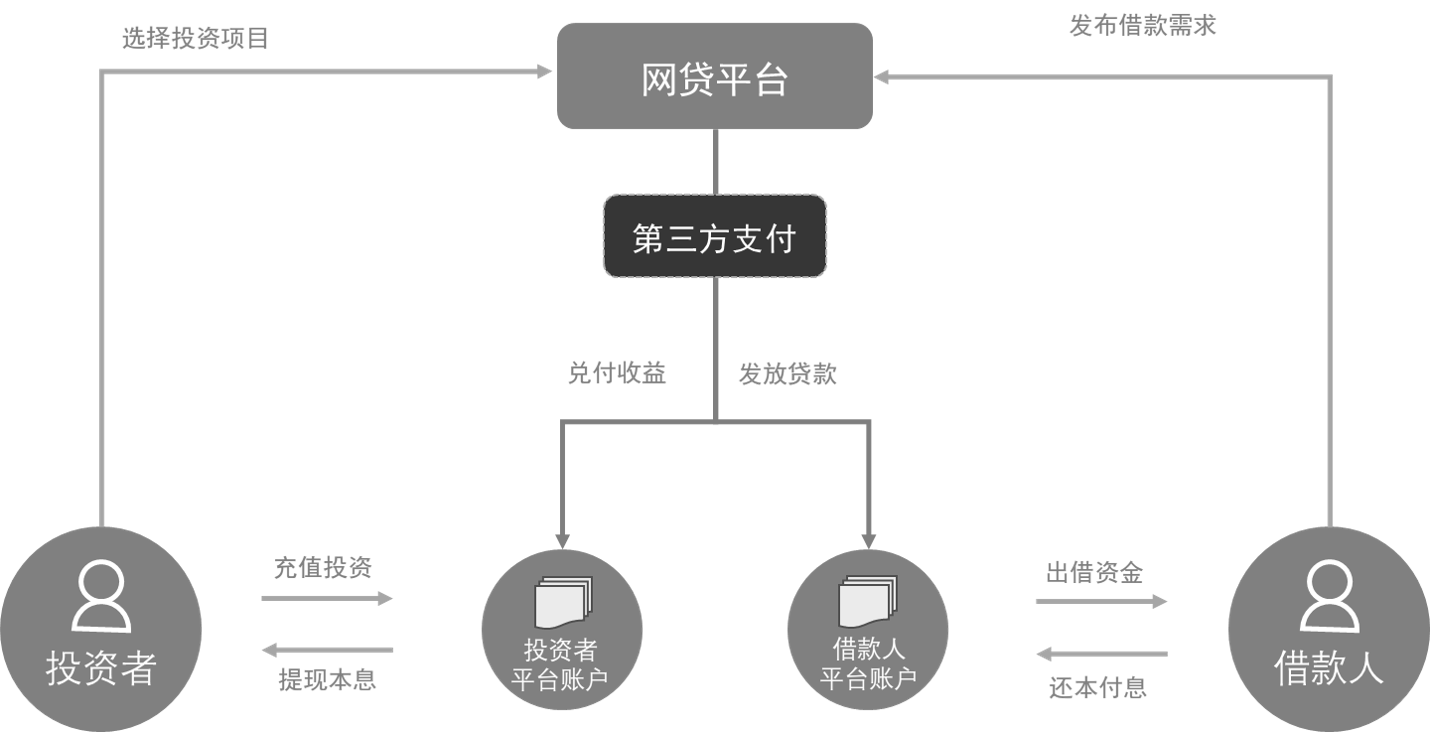
\includegraphics[width=0.7\textwidth]{nobank.png}
\caption{ 网贷平台的早期运营模式(无存管模式)\label{fig:nobank}}
\end{figure}

在这种无银行存管的运营模式下,网贷平台能够直接触碰到投资者和借款人的资金,客户资金可能被直接挪用,因此这种做法也是之后的监管政策明令禁止的。而 P2P 银行存管实际上就是要求由银行存管资金,平台管理交易,做到资金与交易的分离,使得平台无法直接接触资金。图~\ref{fig:bank} 刻画了银行存管下网贷平台的运营模式。

\begin{figure}
\centering
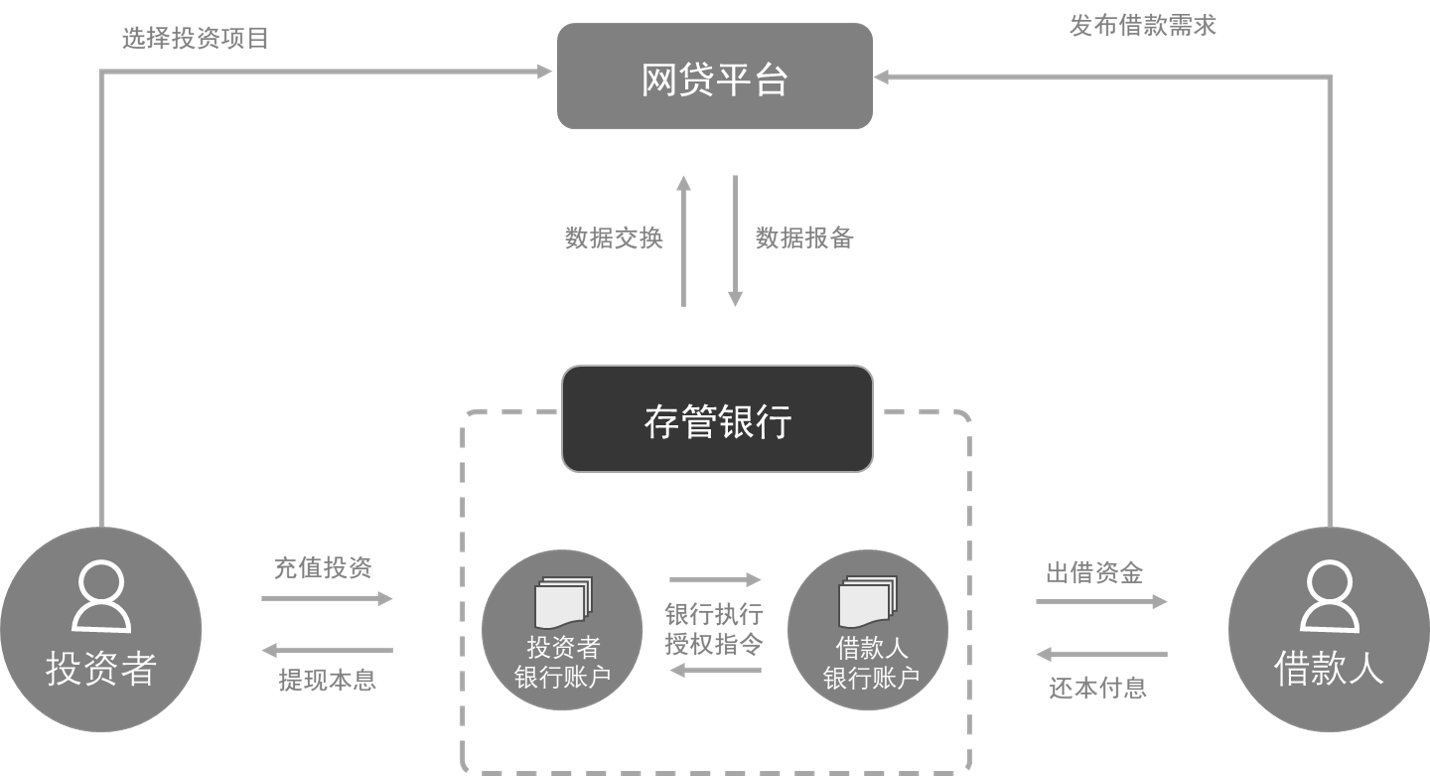
\includegraphics[width=0.7\textwidth]{bank.png}
\caption{银行存管下网贷平台的运营模式\label{fig:bank}}
\end{figure}

存管模式下,投资者和借款人需要在存管银行开设自己独立的银行账户。借款人仍然通过网贷平台发布借款需求,而投资者通过平台进行投资项目的选择,但是与无存管模式的区别在于,平台不能随意对借款人的借款需求进行打包,期限错配也是不允许的,网贷平台仅仅作为信息中介撮合借款人和投资者。在投资者选择投资项目之后,网贷平台将数据发送给存管银行,由银行从投资者存管银行独立账户中将资金划转到借款人存管银行独立账户中,该操作完成后,存管银行再将交易信息返回给网贷平台。投资者可以通过自己的存管账户进行充值提现等操作,而借款人可以从存管账户获得出借资金,到期之后还本付息。整个交易的资金流转不经网贷平台账户,隔绝了平台触碰资金的可能性。与早期网贷平台的无存管模式最大的区别就在于,网贷平台必须转变角色,从金融信用中介转为信息中介,平台只能负责撮合投资者和借款人,而不能参与资金来往。

之所以早期的 P2P 借贷会频繁涉及非法集资、旁氏骗局、诈骗跑路等问题,一个技术上的直接原因就是平台资金没有存管。而银行存管一方面解决了平台的资金流管理问题,可以防止平台自融或资金池的出现,另一方面银行存管有利于平台交易操作正规化、运营信息透明化,能够有效降低平台跑路风险。当然,本质上银行存管对于标的的质量并不做任何审核或担保,所以银行存管只能防止平台直接触碰资金,但无法改变借款人造假、违约等风险。

\subsection{银行存管的进展}
根据网贷之家数据,截至 2018 年 10 月底,全国有 1435 家(不含 445 家问题平台,但包括 34 家问题较多但仍在运营的平台)网贷平台直接与银行对接进行资金存管,涉及 30 个省市\footnote{根据网贷天眼数据,截止到 2019 年 5 月 15 日,总共有 933 家平台完成银行存管,其中正常平台为 626 家,问题平台为 307 家,问题比率为 32.9\%。}。其中,银行资金存管已经上线的网贷平台有 1117 家,已签订银行存管协议但存管业务还未上线的网贷平台有 318 家。

为了考察平台是否真实上线银行存管使用了中国互联网金融协会网站所公示的银行存管信息,其最大优势是该网站上银行存管数据为存管银行所披露,比平台自身披露更加客观可信,也是目前唯一可得的披露了银行存管签订时间与全量业务上线时间的数据来源。截至 2018 年 12 月 4 日,中国互联网金融协会已公示了 29 家银行对接的 561 家 P2P 平台存管信息。其中有 88 家平台已签约但未上线全量业务,占比约为 15.6\%。

\begin{figure}
\centering
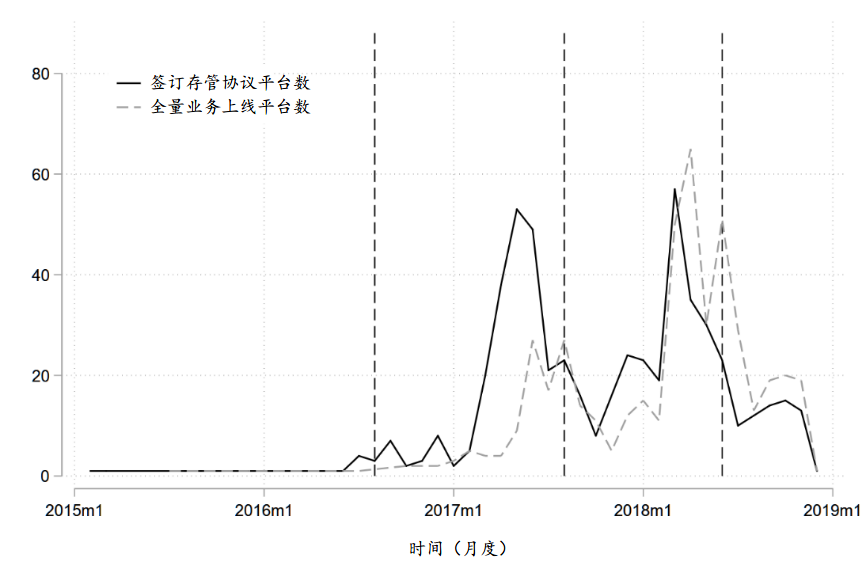
\includegraphics[width=0.7\textwidth]{process.png}
\caption{银行存管的签约时间和全量业务上线时间分布\label{fig:process}}
\end{figure}

从图~\ref{fig:process} 中可以看到在《暂行办法》出台(2016 年 8 月 24 日)之后,有一批平台选择与银行签订存管协议,但是在第一次备案延期之前(2017 年 8 月 24 日),仍然有很大一部分签订协议但是未上线的平台。而后不管选择签订协议或者上线全量业务的平台数量都急剧下降。这说明很可能大部分平台都是为了备案选择紧急签订存管协议。在第二次备案验收时间点前(2018 年 6 月 30 日),不管签订协议还是上线全量业务的平台数目都增加很快,而且同期全量业务上线的平台数比签订协议的平台数更多。而在第二次备案延期之后,无论是签订存管协议的平台数还是上线全量业务的平台数都在下降。

2018 年中国互联网金融协会组织了第三方机构,采取现场与非现场测评相结合的方式,对相关商业银行网贷存管业务流程与技术系统的合规性、完整性进行了测评。同年 9 月 20 日,中国互联网金融协会在“全国互联网金融登记披露服务平台”公示了北京银行等 25 家银行“关于个体网络借贷资金存管系统通过测评声明”,标志着首批通过协会测评的存管银行名单正式出炉。之后,中国互联网金融协会陆续更新了存管银行白名单,目前白名单总共涵盖了 42 家银行。

2018 年 8 月 17 日,全国网贷整治办下发《P2P 合规检查问题清单》的第 66 条明确,“网贷机构未完成与银行业金融机构的资金存管(包含仅签订存管协议但业务未上线运行、业务未全部上线、存管银行未通过测评)”被认定为不合规,该文件还规定了 2018 年 12 月底为 P2P 完成合规检查的最后期限。

\section{银行存管增信作用与中介性质检验}

\subsection{银行存管平台与非银行存管平台的差异}

研究使用了以下四个数据集:
\begin{enumerate*}[label=(\arabic*)]
    \item 网贷之家网站各个网贷平台的运营数据,涉及从 2014 年 11 月至 2018 年 7 月,共计 839 家网贷平台的(周)非平衡面板数据;
    \item 网贷天眼上网贷平台的银行存管信息,包括 762 家网贷平台存管时间以及 57 家存管银行;
    \item 中国互联网金融协会公示的银行存管信息,内容涉及 29 家存管银行共计 561 家网贷平台的银行存管时间以及全量业务上线时间;
    \item 中国互联网金融协会公示的银行测评信息(存管银行白名单)。
\end{enumerate*}
网贷之家上网贷平台的运营数据的核心变量如表~\ref{tab:var} 所示。

\begin{table}[htbp]
  \centering
  \caption{核心变量与定义}
    \begin{tabular}{lll}
    \toprule
    变量    &变量名 & 变量描述 \\
    \midrule
    平均利率  & $interest$ & 一周内平台投资产品的加权平均利率(单位:\%)\\
    平均期限  & $term$  &一周内平台投资产品期限的加权平均(单位:月) \\
    成交量   & $volume$ & 一周内平台的成交量(单位:万元) \\
    资金净流入 & $net\_flow$ & $=$ 投资总额 $-$ 本周内向投资者的还款金额(按本金计,单位:万元) \\
    实还本金  & $repayment$ & $=$ 投资总额 $-$ 本周平台资金净流入(按本金计,单位:万元) \\
    \bottomrule
    \end{tabular}%
  \label{tab:var}%
\end{table}%


需要注意的是,网贷之家并没有提供“实还本金”这个变量。所谓实本金,是指一周内平台向投资者返还的本金数额。由于平台一周内的资金净流入就等于成交量减去实还本金,所以可以利用平台提供的资金净流入和成交量这两上变量推算出实行本金的数额。并且删除了平均利率超过 100 的样本,以及平均期限超过 $100$ 个月的样本。实还本金将作为度量平台待还压力的指标。

网贷平台运营数据中,非存管平台共有 380 家,样本量为 28544,存管平台有 459 家,样本量为 50379。非存管平台相对于存管平台有更高的利率,更短的期限,并且规模更小,待还金额也更小。经过检验,非存管平台与存管平台在平均利率,平均期限,成交量,资金净流入,待还本金等变量之间的差异在 1\% 水平下显著。

\subsection{银行存管的增信作用}

待检验的第一个问题是银行存管是否具有增信作用。也就是说,网贷平台进行银行存管之后,在投资者看来平台是否就变得更加可信?为此,需要检验在给定其它条件不变时,平台在完成银行存管后是否能够吸引更多的投资,即平台成交量是否上升。对应的回归方程如~\eqref{eq:vol} 式所示:
\begin{equation}\label{eq:vol}
volume_{it} = \alpha + \beta bank\_custody_{it} + \gamma x_{it} + f_i + f_t + \varepsilon_{it}
\end{equation}

其中 $volume_{it}$ 是 $i$ 平台在第 $t$ 周的成交量,$bank\_custody_{it}$ 为平台 $i$ 在第 $t$ 周的银行存管状态,如果平台签订了银行存管协议或者全量业务上线,则  $bank\_custody_{it} = 1$。$x_{it}$ 为其他的控制变量(平均利率,平均期限),  $f_i$ 和  $f_t$ 分别为平台的固定效应和时间固定效应(周)。回归结果如表~\ref{tab:volreg} 所示。

\begin{table}[htbp]
  \centering
    \addtolength{\leftskip} {-1cm}
    \addtolength{\rightskip}{-1cm}
  \caption{银行存管与平台成交量}
    \begin{tabular}{lccccccc}
    \toprule
          & (1)   & (2)   & (3)   & (4)   & (5)   & (6)   & (7) \\
    \midrule
    平均利率  & 261.00*** & 264.17*** & 250.92*** & 154.99*** & 642.95*** & 632.91*** & 631.61*** \\
          & (61.57) & (64.64) & (73.95) & (27.49) & (224.98) & (225.70) & (224.83) \\
    平均期限  & -722.26*** & -782.69*** & -846.20*** & -43.37** & -1685.02*** & -1690.49*** & -1689.58*** \\
          & (33.33) & (35.30) & (39.41) & (20.49) & (82.03) & (82.29) & (81.97) \\
    天眼存管  &       & 2418.71*** & 2805.03*** & -241.97 &       &       &  \\
          &       & (395.19) & (457.97) & (153.15) &       &       &  \\
    存管协议  &       &       &       &       & 9996.30*** &       & 12243.70*** \\
          &       &       &       &       & (904.40) &       & (999.27) \\
    全量业务  &       &       &       &       &       & -49.59 & -5842.70*** \\
          &       &       &       &       &       & (1006.22) & (1108.27) \\
    常数项   & 3609.49 & 4275.89 & 5297.68 & -59.92 & -1536.91 & -1249.26 & -1358.88 \\
          & (22633.24) & (23405.48) & (25185.84) & (3344.30) & (34836.60) & (34946.43) & (34812.53) \\
    观测值   & 50382 & 46883 & 40332 & 6551  & 19689 & 19689 & 19689 \\
    $R^{2}$    & 0.02  & 0.02  & 0.03  & 0.16  & 0.05  & 0.04  & 0.05 \\
    平台数   & 459   & 426   & 367   & 59    & 177   & 177   & 177 \\
    平台固定效应 & YES   & YES   & YES   & YES   & YES   & YES   & YES \\
    周固定效应 & YES   & YES   & YES   & YES   & YES   & YES   & YES \\
    平台范围  & 全部平台  & 存管平台  & 正常平台  & 问题平台  & 协会名单  & 协会名单  & 协会名单 \\
    \bottomrule
    \end{tabular}%
  \label{tab:volreg}%
\end{table}%


首先,第(1)列,同时加入平均利率和平均期限,可以看到,随着利率提高,期限缩短,投资者购买的平台产品显著增加。接下来考虑三个用于度量平台是否具有银行存管的指标:
\begin{enumerate*}[label=(\arabic*)]
    \item 天眼存管\footnote{由于网贷天眼上“存管时间”并不区分存管协议的签订和全量业务上线时间,并且,网贷天眼上拥有存管信息的平台比中国互联网金融协会上的平台更多,所以天眼存管也被列入存管的指标。}。根据平台在网贷天眼上披露的建立银行存管的时间,对该变量在存管后取值为 1,存管前取值为 0。不过,网贷天眼中的存管时间并不区分存管协议的签订和全量业务上线时间。
    \item 存管协议。根据中国互联网金融协会公示的银行存管信息,该变量在平台签订了存管协议之后取值为 1,否则为 0;
    \item 全量业务。与变量存管协议的信息来源相同,网贷平台全量业务上线银行存管之后,全量业务取值为 1,否则为 0。
\end{enumerate*}

根据列(2),总体而言,平台拥有银行存管之后成交量显著增加。根据平台在事后是否成为问题平台,(3)、(4)两列对样本进行了区分。可以看到,只有对于正常平台,银行存管才能够增加平台的成交量。(5)--(7)中的三列进一步区分了存管协议签订和全量业务上线。如果分开来单独控制的话,存管协议的签订对于平台而言增信作用明显,而平台上线全量业务,平台的成交量并不受影响。如果同时控制存管协议与全量业务上线,就会发现全量业务上线反而不利于平台吸引投资。这很可能是因为众多平台借助于签订存管协议起到宣传效果,但是,投资者并不希望平台作为信息中介,因而银行存管的全量业务上线之后,投资热情反而下降。这一点可以通过对比部分网贷平台存管账户和非存管账户的情况加以说明。注意到:一方面,平台有了银行存管之后,平台越来越合规,账户资金更安全,不用收管理费提现费等等;但是,另外一方面,相对于非存管账户而言,存管账户的注册、充值、提现均更加繁琐,这导致平台存管之后带来的用户体验下降。另外,部分平台给非存管账户使用者提供投资红包和加息券等优惠,也可能是导致全量业务上线后存管标的投资量下降的原因。

\subsection{平台的信息中介性质检验}

在 2016 年 8 月 24 日《暂行办法》出台之后,网络借贷平台发生的最大改变就是平台性质的转变,也就是平台从金融中介(或信用中介)的性质转变为信息中介。

所以非常重要的一个问题是,在《暂行办法》出台之后,如何判定平台是否是信息中介?暂行办法只是规定了平台必须转型为信息中介,但是,平台实际上作为信用中介存在着还是已经转型为信息中介,投资者很难识别。接下来考察银行存管作为合规最重要也是最基础的验收标准,能否作为平台作为信息中介的一个凭据?又或者有其他的判定标准?

考虑银行存管的原因是,在《暂行办法》出台之后,银行存管变为必须满足的条件之一。以前银行存管作为平台安全性的宣传手段之一,也存在其他类型的存管,特别是联合存管,即便网贷平台有了资金存管或者银行存管,平台实际上仍然拥有资金账户的调配权。现如今,银行存管为合规的条件之一,银行存管的意义发生了改变,特别是在银行存管白名单公布之后之后,银行存管实际上为平台资金上了一把锁。

在《暂行办法》出台之前,由于网贷平台作为金融信用中介的形式存在,平台也会使用期限错配,在面临兑付压力比较大的时候通常会有一些策略行为,比如提高产品的利率、缩短产品的期限、返现红包等~\citep{ddscz2019}。

通过这些策略性行为,平台可以获得更多的投资总额,用于缓解平台的资金压力(现金流压力)。但是在政策后,新设立银行存管的平台一方面平台合规要求更高,另外一方面银行也能作为提供震慑的作用,原因在于,平台的信息,资金交易都在银行有记录,如果平台存疑,监管部门想查这个平台,则会非常容易就能查出来。如果一个平台都是合规操作,并且,进行了银行存管,则一般来说,在平台遇到资金流压力的时候,平台是不会改变产品的特征,因为作为信息中介,平台并没有担保的义务,借款人还不上,平台会通过催收等手段进行贷后处理。但是,催收无果之后投资人需要自行承担其中的损失。并且,对于一个相对成熟,专业的平台,其产品比较稳定。因此需要看在政策前后(政策前银行存管平台少),银行存管是否会改变平台的策略性行为,借此来看银行存管是否能作为平台作为信息中介的凭据。

为了检验利率与待还压力的关系,设定下面的回归方程:
\begin{equation}
interest_{it} = \alpha + \beta \log_{10}(repayment + 1)_{i,t+1} + \gamma x_{it} + f_{i} + f_{t} + \varepsilon_{it}
\end{equation}
其中 $interest_{it}$ 是平台 $i$ 在第 $t$ 周新发布产品的平均利率,$\log_{10}(repayment + 1)_{i,t+1}$ 为平台 $i$ 在第 $t$ 周的实际偿还的本金加 1 然后取对数, 为其他的控制变量(平均期限),$f_i$ 和 $f_t$ 分别为平台的固定效应和时间固定效应(周)。由于《暂行办法》出台前后,平台的区别很大,所以最好直接将数据分为两部分进行回归,回归结果见表 ~\ref{tab:policy_before} 和表 ~\ref{tab:policy_after}。 

\begin{table}[htbp]
  \centering
  \caption{政策前:产品平均利率与平台待还压力}
    \begin{tabular}{lcccc}
    \toprule
    Panel A & 全部    & 正常平台  & 问题平台  & 存管 \\
    \midrule
    $F.\log_{10}(\text{实还本金}+1)$ & 0.17*** & 0.10*** & 0.27*** & 0.13*** \\
          & (0.02) & (0.02) & (0.04) & (0.02) \\
    观测数   & 27,573 & 17,393 & 10,180 & 14,021 \\
    $R^{2}$    & 0.23  & 0.29  & 0.19  & 0.29 \\
    平台数   & 715   & 466   & 249   & 375 \\
    \midrule
    Panel B & 天眼存管  & 协会存管  & 协会存管/正常 & 全量业务 \\
    \midrule
    $F.\log_{10}(\text{实还本金}+1)$ & 0.14*** & 0.12*** & 0.12*** & 0.00 \\
          & (0.03) & (0.03) & (0.03) & (0.32) \\
    观测数   & 12,939 & 5,351 & 5,211 & 139 \\
    $R^{2}$    & 0.30  & 0.28  & 0.28  & 0.61 \\
    平台数   & 347   & 145   & 142   & 5 \\
    平台固定效应 & YES   & YES   & YES   & YES \\
    周固定效应 & YES   & YES   & YES   & YES \\
    \bottomrule
    \end{tabular}%
  \label{tab:policy_before}%
\end{table}%

\begin{table}[htbp]
  \centering
  \caption{政策后:产品平均利率与平台待还压力}
    \begin{tabular}{lcccc}
    \toprule
    Panel A & 全部    & 正常平台  & 问题平台  & 存管 \\
    \midrule
    $F.\log_{10}(\text{实还本金}+1)$ & -0.16*** & -0.17*** & -0.09 & -0.22*** \\
          & (0.02) & (0.02) & (0.05) & (0.03) \\
    观测数   & 73,114 & 55,101 & 18,013 & 45,535 \\
    $R^{2}$    & 0.24  & 0.24  & 0.26  & 0.22 \\
    平台数   & 806   & 546   & 260   & 426 \\
    \midrule
    Panel B & 天眼存管  & 协会存管  & 协会存管/正常 & 全量业务 \\
    \midrule
    $F.\log_{10}(\text{实还本金}+1)$ & -0.23*** & -0.11*** & -0.11*** & -0.04 \\
          & (0.05) & (0.03) & (0.03) & (0.04) \\
    观测数   & 13,940 & 18,329 & 18,017 & 2,745 \\
    $R^{2}$    & 0.09  & 0.35  & 0.35  & 0.31 \\
    平台数   & 326   & 171   & 168   & 89 \\
    平台固定效应 & YES   & YES   & YES   & YES \\
    周固定效应 & YES   & YES   & YES   & YES \\
    \bottomrule
    \end{tabular}%
  \label{tab:policy_after}%
\end{table}%


从表~\ref{tab:policy_before} 可以看出,在政策前,待还压力增加时,平台会选择提高新发产品利率,这也是之前所说的为了吸纳更多的投资来缓解兑付压力。如果区分正常平台和潜在问题平台发现,相对于正常平台,问题平台会提高更高的利率来吸纳投资。根据网贷天眼和中国互联网金融协会提供的银行存管信息(签订银行存管协议或者全量业务上线都算),考虑银行存管平台,也发现同样的表现。而如果区分不同存管类型,待还压力和平均利率之间的关系依然稳健,并无太大差异。但是,当限定存管平台在全量业务上线之后的样本,发现,平均利率和待还压力并没有关系。不过,因为这个样本量比较小,只有 5 个平台,因此这个结果并不能作为判定标准。

而从表~\ref{tab:policy_after} 看出,在政策之后,当平台面临比较大的未来待还时,平台倾向于降低新发布产品的利率(负号和网贷平台压缩平台存量、减小规模的双降政策\footnote{在 2017 年 6 月双降政策出台之后,网贷平台被要求化解存量违规业务、不得新增不合规业务、业务规模不再增加。}有关)。如果区分正常平台和问题平台的话,发现,正常平台仍然会降低利率,但是问题平台并不会,这是因为潜在问题平台并不打算朝着合规方向去整改(合规要求降低待还总额),所以对于问题平台而言,待还压力增加时,并没改变他们发布产品的利率。如果仅仅考虑银行存管平台,待还压力增加时,不论是天眼存管平台,协会存管平台还是在删去问题平台之后,平台会降低平台的利率。而只有在限定存管平台全量业务上线之后,待还压力与利率之间的关系不显著,这实际上说明网贷平台与中国互联网金融协会上的白名单银行签订存管协议之后,并且全量业务上线之后,平台的待还压力和平台新发布的产品的利率特征并无关系。这在一定程度上证明了,即便与白名单银行签订了存管协议也不代表这个平台是作为信息中介存,只有当这个平台全量业务上线之后,这个平台才真正成为了信息中介。

结合之前的回归结果,得出结论:与白名单银行签订了存管协议,并且全量业务上线是唯一评判平台成为了信息中介的标准。而与白名单之外的银行签订存管协议,甚至没有签订协议,都是不可靠的。

\section{结论}
中国互联网金融行业处于转型过程中,借助于网贷天眼、中国互联网金融协会公布的网贷平台银行存管信息,以及网贷平台的微观运营数据,基于投资者的投资决策围绕着银行存管回答了下面几个问题。第一,银行存管是否具有增信作用?如果有,是否存在异质性?第二,银行存管协议与全量业务上线有什么不同的影响?第三,判定网贷平台作为信息中介的依据是什么?
通过对非平衡面板数据的实证回归发现:银行存管确实有增信作用,并且,这个效应与平台与银行签订资金存管协议以及全部业务上线存管有关。根据网贷平台在面对兑付压力时的反应,文章检验了网贷平台的中介性质,发现,只有当网贷平台与存管银行白名单的银行签订存管协议并且全量业务上线,平台才真正成为了信息中介。

这些发现为认识网贷行业提供了重要的实证依据。尤其是在网贷准备备案的重要阶段,对于银行存管的研究能更好把握银行存管的重要性。作为网贷平台备案的最基础、最重要的标准之一,银行存管确实发挥了它的作用,能够为投资者提供非常重要的保障,但更需要注意的是:签订存管协议并不能说明平台的信息中介性质,更重要的是全量业务的上线。投资者不应盲目地相信平台的银行存管宣传以及高利率产品,而应该在深入了解平台的银行存管之后,更加理性的进行投资。但需要注意的是,平台的信息中介性质并不能保证平台/投资的绝对安全,银行存管只能为投资者的资金流提供保障,但是标的是否真实,借款人是否违约这些都需要投资者自行判断。

银行存管对于平台的影响具有很大的异质性,这可能使得无法成功转型的平台会因此退出网贷行业。纯信息中介模式确实有助于隔离用户资金和平台资金,但是,对于网贷平台以及网贷行业的发展到底利弊如何,国内缺乏相关的研究,政策制定者应当在充分把握行业风险之后,逐步推进网贷行业的整改。其中的启示是:政策制定者在保护投资者利益的同时,需要更好的把握网贷行业的发展方向,制定符合中国网贷行业健康发展的政策,让互联网金融的普惠作用发挥的更好。


\bibliography{reference}

\end{document}
